\section{System Design} % talk about general blackboard system structure

A Blackboard System is a way for distinct agents specializing in subproblems to communicate partial solutions and cooperate to find a complete solution. \cite{Corkill2003}
There are three components of a Blackboard System: the Blackboard, the Control, and the Knowledge Sources.
Knowledge Sources are the specialized agents. They examine the Blackboard as input and write their partial solutions on the Blackboard.
The Blackboard is a data structure shared by all the Knowledge Sources and presided over by the Control. It is essentially an open read and write area.
The Control decides which Knowledge Sources run and when the problem has been solved.

\begin{figure}[h]
\centering
	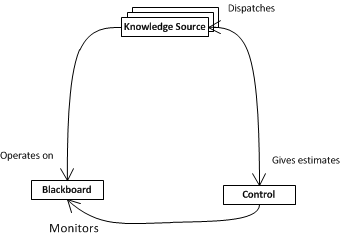
\includegraphics[keepaspectratio=true]{blackboard-system-diagram.png}
\caption{Structure of a general blackboard system}
\end{figure}

\subsection{Blackboard} % talk about the specific blackboard used

For this music composition system, the Blackboard contains two major items: the given musical line, the \emph{cantus firmus}, and the musical line in the progress of composition, the \emph{counterpoint}.
Both the \emph{cantus firmus} and the counterpoint are Voices (see appendix), but the \emph{cantus firmus} is read-only.
The Blackboard also contains other minor, but important, information such as the key or mode of the composition. This is mainly for ease of reference.

\subsection{Knowledge Sources} % talk about the general structure for agents

Knowledge Sources, or agents, embody musical rules or preferences and can range from simple to complex.
Most of Counterpoint is specified by either forbidding certain kinds of musical structures or limiting their use so that others are preferred.
These are respectively known as `hard' and `soft' rules. Ideally, the system should not violate any hard rules and minimize violations of soft rules.
Agents embodying these rules essentially examine a location in a musical line and test whether their rule is upheld or not.
These agents exist to cut off the composition when it progresses in an undesirable way.

The counterpart to these tester agents are generators that modify the composition by extending it or changing an existing portion.
The most basic version of this type of agent just attaches random notes, within the allowed range, to the end of the existing composition.
More complex agents could make sweeping modifications to achieve higher level musical constructs.
For example, an agent could identify regions that are too flat (not enough vertical motion) and make them more contoured.

Generators and testers work together through a feedback loop to create valid compositions.

\begin{figure}[h]
\centering
	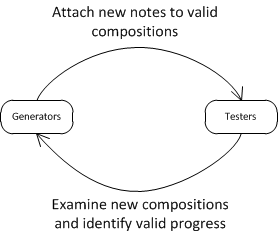
\includegraphics[keepaspectratio=true]{generator-and-tester-dynamic.png}
\caption{The generator and tester agent dynamic}
\end{figure}

\subsection{Control} % talk about the control structure

The Control tracks the history of the Blackboard to help it choose how to precede.
For each version of the Blackboard, the Control records some useful metadata:
  which tests still need to run for a Blackboard,
  the parent of a Blackboard, which is just the Blackboard it was generated from,
  and the number and type of rule violations of a Blackboard and its descendants.
Using this ordering of Blackboards based on rule violations and counterpoint length, 
  the Control operates on the best Blackboard at any given time, 
  running tests and applying generators until it finds a Blackboard that passes the tests and is as long as the \emph{cantus firmus}.

